\section{Descartes Labs}

Descartes Labs використовує власний Python API.  Для %
побудови безхмарних зображень
компанія застосовує дані супутників Landsat 8, %
Sentinel-1 SAR, Sentinel-2 Red Edge, а
також дані аерозйомки, які покривають лише %
територію США.

Під час первинного аналізу карт цієї %
організації виявлено дефектні смуги (рис.
\ref{fig:descartes:b}), тобто різницю значень пікселів %
після склеювання.  На знімках у
деяких регіонах присутня велика кількість %
хмарних пікселів (рис.
\ref{fig:descartes:a}), а також помітна різниця між %
пікселями на стиках знімків.

Таким чином, алгоритм отримання безхмарних %
супутникових знімків Descartes Labs має
недоліки, що впливають на якість результату.

\begin{figure}[H]
  \centering \subfloat[Дефектні зони хмарами]{
    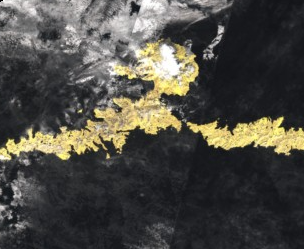
\includegraphics[width=0.35\textwidth,height=0.2\textheight]{images/image2}
    \label{fig:descartes:a}
  } \subfloat[Склейка знімків]{
    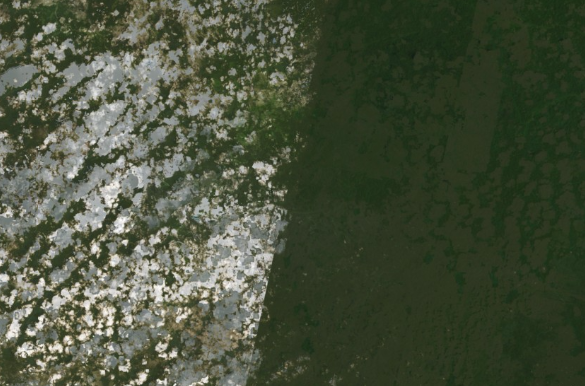
\includegraphics[width=0.35\textwidth,height=0.2\textheight]{images/image1}
    \label{fig:descartes:b}
  } \caption{Супутникові знімки Descartes Labs}
\end{figure}

\section{EOxCloudless}

Іншою компанією, що спеціалізується на обробці %
супутникових даних, є EOxCloudless.  Вона
аналізує дані супутників Sentinel-1 та Sentinel-2 і %
забезпечує моніторинг
сільськогосподарських територій за допомогою %
оптичних і радіолокаційних даних.

\begin{figure}[H]
  \centering \subfloat[Дефектні зони хмарами]{
    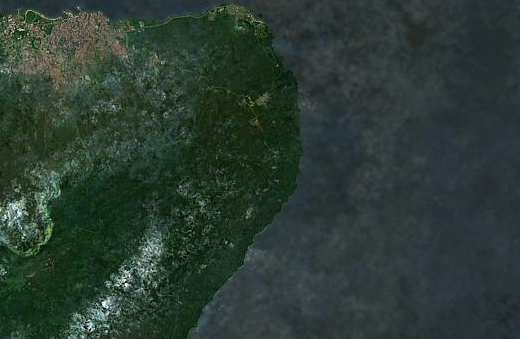
\includegraphics[width=0.35\textwidth,height=0.2\textheight]{images/image4}
    \label{fig:eoxcloudless:a}
  } \subfloat[Склейка знімків]{
    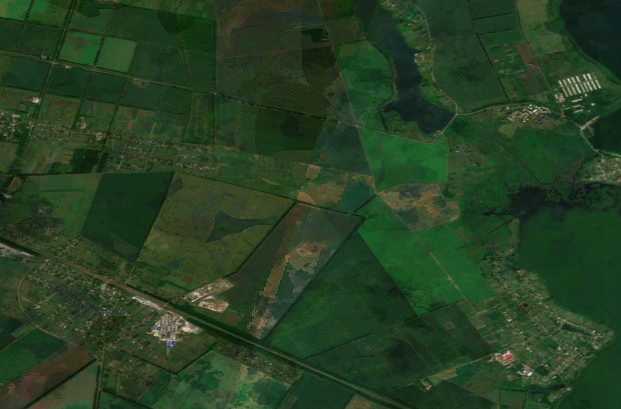
\includegraphics[width=0.35\textwidth,height=0.2\textheight]{images/image3}
    \label{fig:eoxcloudless:b}
  } \caption{Супутникові знімки EOxCloudless}
\end{figure}

На знімках також присутні дефекти (рис.  %
\ref{fig:eoxcloudless:b}), хоч і не в такій
кількості, як на супутникових знімках %
попередньої компанії.  У цьому випадку колірна
різниця між регіонами (рис.  \ref{fig:eoxcloudless:a}) %
помітно менша, тому зображення
виглядає краще.

На основі первинного аналізу результатів %
EOxCloudless та Descartes Labs у деяких
регіонах виявлено неякісні знімки та проблеми %
з відновленням неповних даних.  Україні
потрібна власна безхмарна карта, оскільки вона %
дасть змогу покращити моніторинг посівних
площ і аналіз культур, а також відстежувати %
розливи водойм і річок.

У дипломній роботі описано можливе вирішення %
проблеми неповних даних і створено модель,
яка формує безхмарний супутниковий знімок на %
основі даних сімейства Sentinel-2.  Модель
також може працювати з будь-якими %
триканальними RGB-супутниковими даними.
